\chapter{Geometría Diferencial Sintética}
\label{geodif}

En esta sección usaremos los axiomas que expone Mclarty \cite{mclarty1988defining} para trabajar
rigurosamente con infinitesimales y fundamentar al cálculo, así como al estudio de variedades.
\begin{axioma}[label=ax:gds1]
Existe un espacio, $R$, que cuenta con una estructura de anillo conmutativo con unidad.
\end{axioma}
\begin{axioma}[label=ax:gds2]
El anillo $R$ no es trivial, es decir, $1\not = 0$.
\end{axioma}
\begin{axioma}[label=ax:gds3]
En la lógica interna de $R$, $R$ es un campo.
\end{axioma}
Y el axioma de Kock-Lawvere \cite{lawvere1979categorical}, para el cual es necesario definir
al espacio de infinitesimales $D$, el cual será el igualador de $0\colon R\to R$, el mapa constante $0$, y $(-)^2\colon R\to R$.
Equivalentemente, $D$ es el subespacio (subobjeto) de $R$, $D= \{d \in R\colon d^2=0 \}$.
\begin{axioma}[label=ax:gds4]
$(\forall f \in R^D)(\exists ! b \in R)(\forall d \in D) (f(d) = f(0)+d \cdot b)$.
\end{axioma}
Intuitivamente, \ref{ax:gds4} dice que toda función de $D$ a $R$ es lineal. A continuación 
mostramos algunas propiedades de los infinitesimales y que estos cuatro axiomas ya nos 
permiten hacer cálculo básico.

\section{El espacio de infinitesimales}
Los infinitesimales con los que trabajamos en GDS son números $d\in D$ que al cuadrado dan cero, y por supuesto,
esto implica que todas las potencias mayores a dos también dan cero, pues $d^n=d^2\cdot d^{n-2}=0$ para $n>2$. Esto
corresponde con los argumentos de Newton, Leibniz, Euler, entre otros, donde se eliminan los términos de orden
superior de una cantidad infinitesimal. Sin embargo, si queremos que $R$ sea un campo y tenemos que $\lnot(d=0)$,
$d$ es invertible, por lo que $d^2=0$ implica $d=0$, entonces sucede que $\lnot\lnot(d=0)$, pues estamos usando
lógica constructivista. Por otro lado, si para todo $d\in D$, $d=0$ y fijamos $f\colon  D \to R$, obtenemos que
$f(0)=f(d)=f(0)+d \cdot b$ aplicando \ref{ax:gds4}, pero como $d=0$, $f(d)=f(0)+d \cdot 0=f(0)+d \cdot 1$, y por unicidad
de $b$, $b=0=1$, lo cual es inconsistente con \ref{ax:gds2}. Así que también $\lnot (\forall d \in D)(d=0)$ es verdad.
De esta manera, $R$ puede ser un campo a pesar de los infinitesimales, en el sentido de que $\lnot(r=0)\implies \exists s\in R(s\cdot r=1)$.

\section{Infinitesimales y Microcancelación}
Si resulta que $(\forall d \in D) (d\cdot r = d\cdot s)$ con $r,s\in R$, podemos concluir
$r=s$. Demostración: Definimos $f\colon  D\to R$ como $f(d)=d\cdot r = d\cdot s$, luego,
por \ref{ax:gds4}, $f(d) = f(0)+d\cdot b$ donde $f(0) = 0\cdot r = 0$, entonces $d\cdot b=d\cdot r = d\cdot s$
con $b$ única. Por lo tanto, $r=b=s$.

\section{Operaciones con infinitesimales}
Si $r\in R$ y $d\in D$, entonces $d\cdot r \in D$, porque $(d\cdot r)^2=d^2\cdot r^2=0\cdot r^2=0$.
Si $d_1\in D$ y $d_2\in D$, entonces $(d_1+d_2)^2=d_1^2+2\cdot d_1\cdot d_2+d_2^2=2\cdot d_1\cdot d_2$.

\section{La derivada y reglas básicas}
Sea $f\colon  R\to R$, consideramos a $g\colon  D\to R$ tal que $g(d)=f(a+d)$ para alguna
$a\in R$ fija. Por \ref{ax:gds4}, $f(a+d)=g(d)=g(0)+d\cdot b$, pero $g(0)=f(a+0)=f(a)$, entonces
$f(a+d)=f(a)+d\cdot b$ y definimos a $b$ como la derivada de $f$ en $a$, $f'(a)$. Dado que $a$ era
arbitrario, en realidad definimos a una función $f'\colon  R \to R$, la derivada de $f$, que
puede volver a ser diferenciada con el mismo procedimiento. Concluimos que todas las funciones
de $R$ en $R$ son suaves.

\begin{definition}[label=def:derivada]
  Sea $f\colon  R\to R$ y $a\in R$. Definimos $f'(a)$ como el único número tal que para todo $d\in D$
  \begin{equation*}
    f(a+d)=f(a)+d\cdot f'(a)
  \end{equation*}
  Notemos que si pudiéramos dividir entre $d$, tendríamos $f'(a) = \frac{f(a+d)-f(a)}{d}$, lo cual es la definición clásica de derivada.
\end{definition}

% {\color{red}Borrar esto después. Ahora se puede hacer referencia a lo que
% definas o enuncies, ver definición~\ref{def:defrivada} o el teorema~\ref{thm:reglasderivada}.}

\begin{theorem}[label=thm:reglasderivada]
  Si $f\colon  R\to R$,\ $g\colon  R\to R$,\ $a,c\in R$ y $d\in D$, entonces
\begin{enumerate}[label=\textbf{\alph*)}]
    \item $c' = 0$
    \item $(c\cdot f)' =c\cdot f'$
    \item $\id' = 1$
    \item $(f+g)'=f'+g'$
    \item $(f\circ g)' =(f'\circ g)\cdot g'$
    \item $(f\cdot g)' =f'\cdot g+f\cdot g'$
\end{enumerate}
\end{theorem}
\begin{proof}
  Probemos d) como ejemplo. $(f+g)(a+d) = f(a)+g(a)+d\cdot (f+g)'(a)$
  por definición de derivada, pero también $(f+g)(a+d) = f(a+d)+g(a+d)=f(a)+d\cdot f'(a)+g(a)
  +d\cdot g'(a)$. Cancelando términos comunes obtenemos $d\cdot (f+g)'(a) = d \cdot[f'(a)+g'(a)]$
  y por microcancelación, $(f+g)'(a)=f'(a)+g'(a)$ con $a$ cualquiera, entonces
  $(f+g)'=f'+g'$.
  
  Para demostrar a) consideremos
  \begin{align*}
   c(a+d) &= c(a)+d\cdot c'(a)\\
    c &= c+d\cdot c'(a)\\
    d\cdot 0 &= d\cdot c'(a)\\
    c'(a) &= 0\\
    c' &= 0
  \end{align*}

  Ahora, para mostrar el inciso b), tenemos que
  \begin{align*}
     (c\cdot f)(a+d) &= c\cdot f(a)+d\cdot (c\cdot f)'(a)\\
      f(a+d) &= f(a)+d\cdot f'(a)\\
      c\cdot f(a+d) &= c\cdot f(a)+ c\cdot d\cdot f'(a)\\
      d\cdot [c\cdot f'(a)] &= d\cdot (c\cdot f)'(a)\\
      (c\cdot f)'(a) &=c\cdot f'(a)\\
      (c\cdot f)' &=c\cdot f' 
  \end{align*}

  El inciso c) se sigue de:
  \begin{align*}
     \id (a+d) &= \id (a)+d\cdot \id '(a)\\
      a+d &= a+d\cdot \id '(a)\\
      d\cdot 1 &= d\cdot \id '(a)\\
      \id '(a) &= 1\\
      \id ' &= 1\\
  \end{align*}

  Para el inciso e) hacemos lo siguiente
  \begin{align*}
     (f\circ g)(a+d) &= f(g(a))+d\cdot (f\circ g)'(a)\\
      (f\circ g)(a+d) &= f(g(a)+d\cdot g'(a))\\
      (f\circ g)(a+d) &= f(g(a))+[d\cdot g'(a)] \cdot f'(g(a))\\
      d\cdot (f\circ g)'(a) &= d\cdot [f'(g(a))\cdot g'(a)]\\
      (f\circ g)'&=(f'\circ g)\cdot g'\\
  \end{align*}

  Finalmente, para el inciso f) tenemos
  \begin{align*}
     (f\cdot g)(a+d) &= f(a)\cdot g(a)+d\cdot (f\cdot g)'(a)\\
      (f\cdot g)(a+d) &= f(a+d)\cdot g(a+d)\\
      (f\cdot g)(a+d) &= [f(a)+d\cdot f'(a)]\cdot [g(a)+d\cdot g'(a)]\\
      (f\cdot g)(a+d) &= f(a)\cdot g(a)+d\cdot[f'(a)\cdot g(a)+g'(a)\cdot f(a)]+d^2\cdot f'(a)\cdot g'(a)\\
      d\cdot (f\cdot g)'(a)&=d\cdot[f'(a)\cdot g(a)+f(a)\cdot g'(a)]\\
      (f\cdot g)'&=f\cdot g+f\cdot g' \qedhere
  \end{align*}
\end{proof}

\section{Ejemplos}
Sea $f(x) = 5x^2+3$. En ese caso, $f(x+d)=5(x^2+2xd+d^2)+3=5x^2+3+df'(x)$, entonces $d\cdot 10x=d\cdot f'(x)$.
Por tanto, $f'(x)=10x$.

Con axiomas más fuertes podemos introducir números transcendentales y por ejemplo, a la función seno. Para encontrar
la derivada de $seno(x)$, debemos evaluar $seno(a+d)=seno(a)\cdot cos(d)+cos(a)\cdot seno(d)$ con $a\in R$ y $d\in D$. Entonces queremos
saber cuanto valen $cos(d)$ y $seno(d)$, así que hay que considerar un triángulo rectángulo con un ángulo tan pequeño
que vale $d$. Pero a escalas infinitesimales, el círculo se ve como una línea recta, es decir, la longitud de arco para
trazar el ángulo $d$ es tan pequeña que el arco en realidad es una recta y por tanto, si trazamos el triángulo en un círculo unitario, el cateto opuesto al ángulo $d$ también mide $d$.
Ahora, si la hipotenusa es de longitud 1, lo anterior implica que $seno(d)=d$ y $cos(d)=\sqrt{1^2-d^2}=1$. Por lo tanto, $seno(a+d)=seno(a)+d\cdot cos(a)$ y $seno'(a)=cos(a)$
para toda $a\in R$ por \ref{def:derivada}.

\begin{center}
  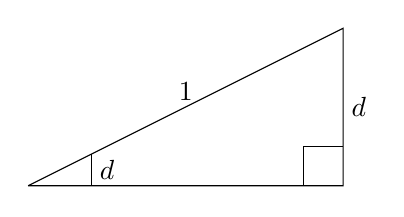
\begin{tikzpicture}
    \draw (1,1) -- (5,1) -- (5,3) -- (1,1);
    \draw (5,1.5) -- (4.5,1.5) -- (4.5,1);
    \draw (1.8,1) -- (1.8,1.4);

    \node at (2,1.2) {$d$};
    \node at (3,2.2) {$1$};
    \node at (5.2,2) {$d$};
  \end{tikzpicture}
\end{center}

\section{Más axiomas para Espacios}

\begin{definition}[label=def:discreto]
  Un espacio $E$ es discreto si y solo si es decidible, es decir, $(x=y) \lor \lnot(x = y)$ es verdad con $x,y$ variables
  variando sobre $E$.
\end{definition}

Mclarty le pide más axiomas a Espacios.

\begin{axioma}[label=ax:gds5]
Existe un espacio $N$ que es un objeto de números naturales.
\end{axioma}

Se puede demostrar que $N$ es es un espacio discreto.

\begin{definition}[label=puntos]
Los puntos de un espacio $E$ son sus elementos globales, morfismos de la forma $1\to E$
\end{definition}

\begin{axioma}[label=ax:gds6]
Para todo espacio $E$, $E \cong  0 $ o $E$ tiene al menos un punto.
\end{axioma}

Esto implica que si $b_1, b_2\in B$ entonces $(b_1=b_2)\lor \lnot(b_1=b_2)$ es verdad incluso si $B$ no es discreto.

\begin{axioma}[label=ax:gds7]
Todo espacio $E$ tiene un subespacio $\Gamma E$ discreto tal que todo punto de $E$ está en $\Gamma E$. 
\end{axioma} 